%%%%%%%%%%%%%%%%%%%%%%%%%%%%%%%%%%%%%%%%%%%%%%%%%%%%%%%%%%%%%%%%%%%%%
%% This is a (brief) model paper using the achemso class
%% The document class accepts keyval options, which should include
%% the target journal and optionally the manuscript type. 
%%%%%%%%%%%%%%%%%%%%%%%%%%%%%%%%%%%%%%%%%%%%%%%%%%%%%%%%%%%%%%%%%%%%%
\documentclass[journal=jacsat,manuscript=article]{achemso}
% \SectionNumbersOn
%\usepackage[letterpaper,left=0.5in,right=0.5in,top=1.0in,bottom=1.0in]{geometry}

%%%%%%%%%%%%%%%%%%%%%%%%%%%%%%%%%%%%%%%%%%%%%%%%%%%%%%%%%%%%%%%%%%%%%
%% Place any additional packages needed here.  Only include packages
%% which are essential, to avoid problems later. Do NOT use any
%% packages which require e-TeX (for example etoolbox): the e-TeX
%% extensions are not currently available on the ACS conversion
%% servers. 
%%%%%%%%%%%%%%%%%%%%%%%%%%%%%%%%%%%%%%%%%%%%%%%%%%%%%%%%%%%%%%%%%%%%%
\usepackage[version=3]{mhchem} % Formula subscripts using \ce{}
\usepackage{siunitx} % generating degrees Celsius in the document 
\usepackage{color}
\usepackage{soul} % allows highlighting text 
\usepackage{makecell}
\usepackage{booktabs}
\usepackage{amsmath}
\usepackage{amssymb}
\usepackage{gensymb}
\usepackage{verbatim}
\usepackage{hyperref}
\hypersetup{
    colorlinks=true,
    citecolor= red,
    linkcolor=blue,
    urlcolor=blue, 
    breaklinks=true
}
\usepackage{ulem}
\usepackage{float}


%%%%%%%%%%%%%%%%%%%%%%%%%%%%%%%%%%%%%%%%%%%%%%%%%%%%%%%%%%%%%%%%%%%%%
%% If issues arise when submitting your manuscript, you may want to
%% un-comment the next line.  This provides information on the
%% version of every file you have used.
%%%%%%%%%%%%%%%%%%%%%%%%%%%%%%%%%%%%%%%%%%%%%%%%%%%%%%%%%%%%%%%%%%%%%
%%\listfiles

%%%%%%%%%%%%%%%%%%%%%%%%%%%%%%%%%%%%%%%%%%%%%%%%%%%%%%%%%%%%%%%%%%%%%
%% Place any additional macros here.  Please use \newcommand* where
%% possible, and avoid layout-changing macros (which are not used
%% when typesetting).
%%%%%%%%%%%%%%%%%%%%%%%%%%%%%%%%%%%%%%%%%%%%%%%%%%%%%%%%%%%%%%%%%%%%%
\newcommand*\mycommand[1]{\texttt{\emph{#1}}}
\DeclareRobustCommand
  \Compactcdots{\mathinner{\cdotp\mkern-2mu\cdotp\mkern-2mu\cdotp}}

%%%%%%%%%%%%%%%%%%%%%%%%%%%%%%%%%%%%%%%%%%%%%%%%%%%%%%%%%%%%%%%%%%%%%
%% Meta-data block
%% ---------------
%% Each author should be given as a separate \author command.
%%
%% Corresponding authors should have an e-mail given after the author
%% name as an \email command. Phone and fax numbers can be given
%% using \phone and \fax, respectively; this information is optional.
%%
%% The affiliation of authors is given after the authors; each
%% \affiliation command applies to all preceding authors not already
%% assigned an affiliation.
%%
%% The affiliation takes an option argument for the short name.  This
%% will typically be something like "University of Somewhere".
%%
%% The \altaffiliation macro should be used for new address, etc.
%% On the other hand, \alsoaffiliation is used on a per author basis
%% when authors are associated with multiple institutions.
%%%%%%%%%%%%%%%%%%%%%%%%%%%%%%%%%%%%%%%%%%%%%%%%%%%%%%%%%%%%%%%%%%%%%
\author{Stephen P. Vicchio}
\affiliation[Clemson University]
{Department of Chemical and Biomolecular Engineering, Clemson University, Clemson, SC}
\author{Zhihengyu Chen}
\affiliation[Stony Brook University]
{Department of Chemistry, Stony Brook University, Stony Brook, NY}
\author{Karena W. Chapman}
\email{karena.chapman@stonybrook.edu}
\affiliation[Stony Brook University]
{Department of Chemistry, Stony Brook University, Stony Brook, NY}
\author{Rachel B. Getman}
\email{rgetman@clemson.edu}
\affiliation[Clemson University]
{Department of Chemical and Biomolecular Engineering, Clemson University, Clemson, SC}

%%%%%%%%%%%%%%%%%%%%%%%%%%%%%%%%%%%%%%%%%%%%%%%%%%%%%%%%%%%%%%%%%%%%%
%% The document title should be given as usual. Some journals require
%% a running title from the author: this should be supplied as an
%% optional argument to \title.
%%%%%%%%%%%%%%%%%%%%%%%%%%%%%%%%%%%%%%%%%%%%%%%%%%%%%%%%%%%%%%%%%%%%%
\title[manuscript]{
Computational and Experimental Characterization of the Ligand Environment of a \ce{Ni4} Cluster Supported on a Metal-Organic Framework
}

%%%%%%%%%%%%%%%%%%%%%%%%%%%%%%%%%%%%%%%%%%%%%%%%%%%%%%%%%%%%%%%%%%%%%
%% Some journals require a list of abbreviations or keywords to be
%% supplied. These should be set up here, and will be printed after
%% the title and author information, if needed.
%%%%%%%%%%%%%%%%%%%%%%%%%%%%%%%%%%%%%%%%%%%%%%%%%%%%%%%%%%%%%%%%%%%%%
\abbreviations{IR,NMR,UV}
\keywords{American Chemical Society, \LaTeX}

%%%%%%%%%%%%%%%%%%%%%%%%%%%%%%%%%%%%%%%%%%%%%%%%%%%%%%%%%%%%%%%%%%%%%
%% The manuscript does not need to include \maketitle, which is
%% executed automatically.
%%%%%%%%%%%%%%%%%%%%%%%%%%%%%%%%%%%%%%%%%%%%%%%%%%%%%%%%%%%%%%%%%%%%%
\begin{document}

%%%%%%%%%%%%%%%%%%%%%%%%%%%%%%%%%%%%%%%%%%%%%%%%%%%%%%%%%%%%%%%%%%%%%
%% The "tocentry" environment can be used to create an entry for the
%% graphical table of contents. It is given here as some journals
%% require that it is printed as part of the abstract page. It will
%% be automatically moved as appropriate.
%%%%%%%%%%%%%%%%%%%%%%%%%%%%%%%%%%%%%%%%%%%%%%%%%%%%%%%%%%%%%%%%%%%%%
%\begin{tocentry}
%
%Some journals require a graphical entry for the Table of Contents.
%This should be laid out ``print ready'' so that the sizing of the
%text is correct.
%
%Inside the \texttt{tocentry} environment, the font used is %Helvetica
%8\,pt, as required by \emph{Journal of the American Chemical
%Society}.
%
%The surrounding frame is 9\,cm by 3.5\,cm, which is the maximum
%permitted for  \emph{Journal of the American Chemical Society}
%graphical table of content entries. The box will not resize if the
%content is too big: instead it will overflow the edge of the box.
%
%This box and the associated title will always be printed on a
%separate page at the end of the document.
%
%\end{tocentry}

%%%%%%%%%%%%%%%%%%%%%%%%%%%%%%%%%%%%%%%%%%%%%%%%%%%%%%%%%%%%%%%%%%%%%
%% The abstract environment will automatically gobble the contents
%% if an abstract is not used by the target journal.
%%%%%%%%%%%%%%%%%%%%%%%%%%%%%%%%%%%%%%%%%%%%%%%%%%%%%%%%%%%%%%%%%%%%%
\begin{abstract}
Heterogeneous catalysts exhibit dynamic changes in structure and composition as a function of operating conditions that impact on catalytic performance. For traditional bulk metal heterogeneous catalysts, the relationships between operating conditions and composition/structure are well documented. However, these same trends remain unestablished for single-site heterogeneous catalysts (SSHCs). The active site is a small metal clusters anchored to a solid support, which leads to improved metal utilization and increased active site tunability compared to traditional bulk metal catalysts. Here we focus on one such SSHC composed of a 3d transition metal complex (i.e., \ce{Ni_4O_xH_y}) supported on a porous metal-organic framework (MOF). We investigate the ligand environment of the \ce{Ni4} cluster supported on the NU-1000 MOF (Ni-NU-1000) as the \ce{Ni} ion ligand environment varies from \ce{OH}, \ce{H2O}, \ce{O}, and \ce{H} ligands by combining pair distribution function (PDF) and \textit{ab initio} thermodynamic analysis. Phase diagrams from thermodynamic modeling show the ligand composition at different conditions, while simulated PDFs for optimized configurations allow their local atomic structure to be compared to experimental PDF data. We find that \ce{Ni4} clusters with \ce{Ni} coordination numbers comparable to those observed experimentally are surrounded by a significant number \ce{OH} and \ce{H2O} ligands and occur at high \ce{H2O} chemical potential. Additionally, differential PDF analysis suggests that asymmetries in the \ce{Ni} ligand environment of an individual cluster or a distribution of \ce{Ni} clusters within Ni-NU-1000 that contain different \ce{H2O} content explain structural features seen in the experimental d-PDFs. The combined modeling approach provides new insights into the \ce{Ni} coordination environment for Ni-NU-1000, and demonstrate how SSHC active site structure is sensitive to different conditions. 
\end{abstract}

%%%%%%%%%%%%%%%%%%%%%%%%%%%%%%%%%%%%%%%%%%%%%%%%%%%%%%%%%%%%%%%%%%%%%
%% Start the main part of the manuscript here.
%%%%%%%%%%%%%%%%%%%%%%%%%%%%%%%%%%%%%%%%%%%%%%%%%%%%%%%%%%%%%%%%%%%%%

\section{Introduction}
%%%%%%%%%%%%%%%%%%%%%%%%%%%%%%%%%%%%%%%%%%%%%%%%%%%%%%%%%%%%%%%%%%%%%
%% Introduction
%%%%%%%%%%%%%%%%%%%%%%%%%%%%%%%%%%%%%%%%%%%%%%%%%%%%%%%%%%%%%%%%%%%%%

Single-site heterogeneous catalysts (SSHCs)\cite{Thomas2005} offer improved metal utilization and well-defined active site structures\cite{Qiao2011, Cui2017, Yang2013} compared to traditional bulk heterogeneous metal catalysts. These catalysts can be anchored to a variety of solid supports,\cite{Hlatky2000, Kaiser2020, Wasson2019} such as metal-organic frameworks (MOFs),\cite{Zheng2019, AbdelMageed2019, Huang2019} covalent-organic frameworks (COFs),\cite{Zhong2019, Romero-Muniz2020} zeolites,\cite{Mao2016, Kistler2014} and metal\cite{Patel2019, Pei2017, Jiao2019} and metal oxide surfaces.\cite{Bo2019, Riley2018, Tang2019} In many cases, SSHCs are anchored to the support via organic ligands, which strongly influence the chemical reactivity and selectivity,\cite{DeRita2019} similar to homogeneous catalysts.\cite{Rogge2017} 

Also similar to homogeneous catalysts is the appeal of tuning ligand environments to promote challenging chemistries.\cite{Desai2018} For example, novel SSHCs with tuned ligand environments have been used in the site-selective borylation and silylation of \textit{sp}$^{3}$ bonds\cite{Manna2016} and in the tandem oxidation and functionalization of styrene.\cite{Beyzavi2015} However, like heterogeneous catalysts, the ligand environment of SSHCs depends on catalytic operating conditions, which makes it hard to predict.\cite{Shi2021} While extensive research over the last several decades has garnered significant intuition about the influence of catalytic operating conditions on the compositions and structures of heterogeneous catalysts,\cite{Getman2008, Miller2011, Ranea2008, Heard2016, Bray2014, Ganzler2017} the same intuition for SSHCs does not exist.\cite{Mandal2020, Felvey2022, Giewont2021, Mesilov2021} This lack of knowledge hinders the design of SSHCs, particularly for carrying out challenging chemistries.\cite{Liu2019} 

In this work, we seek to improve insights about ligand environments of SSHCs under under catalytic operating conditions by characterizing a ligated \ce{Ni} cation catalyst under catalytic hydrogenation conditions. We are interested in hydrogenation conditions because of their importance to the energy industry, with Ni being a prevalent catalyst. For example, the Shell higher olefins process (ethene oligomerization),\cite{1988Reuben} steam reforming of methane,\cite{Ross1973} and various hydrocarbon hydrogenation reactions\cite{Ryabchuk2018} employ ligated Ni cation catalysts. As a model of a ligated \ce{Ni} cation catalyst, we investigate a \ce{Ni} cluster supported on the metal-organic framework (MOF) NU-1000. Prior investigation into this cluster provides clues about the structure and ligand environment that is present under hydrogenation conditions.\cite{Mondloch2013, Li2016sintering} Following installation of the \ce{Ni} cluster (using atomic layer deposition (ALD) in MOFs (AIM)\cite{Mondloch2013}), experimental and computation characterization suggests the \ce{Ni} cluster comprises four \ce{Ni} cations along with oxo- (\ce{O}), hydroxo- (\ce{OH}), water (\ce{H2O}), and hydride (\ce{H}) ligands,\cite{PlateroPrats2017} and that all of these types of ligands potentially participate in the catalysis, with the hydride being suggested as the active site.\cite{Shabbir2020, Li2016sintering, Yeh2021, Brogaard2016} However, questions still remain as to the precise ligand environment, as well as how it influences catalytic performance. 

Herein, we combine pair distribution function (PDF) simulations, density functional theory (DFT) calculations, and \textit{ab initio} thermodynamic modeling to provide insight into the ligand environment of a \ce{Ni} cluster catalyst supported in NU-1000. We find that the \ce{Ni} ions are highly coordinated with \ce{OH}, \ce{H2O}, and possibly \ce{O} ligands, and that hydride ligands are not stable. We further find that ligand arrangements are asymmetric, with different Ni ions comprising different numbers of ligands, or even different ligands altogether. Finally, our results suggests a distribution of ligand environments with subtle differences in the number of ligands. 


\section{Methodology}
%%%%%%%%%%%%%%%%%%%%%%%%%%%%%%%%%%%%%%%%%%%%%%%%%%%%%%%%%%%%%%%%%%%%%
%% Methodology
%%%%%%%%%%%%%%%%%%%%%%%%%%%%%%%%%%%%%%%%%%%%%%%%%%%%%%%%%%%%%%%%%%%%%

\subsection{NU-1000 Structure}
The MOF NU-1000 is comprised of \ce{Zr6(\mu_{3}-O)4(\mu_{3}-OH)4(H2O)4(OH)4} nodes interconnected with tetratopic 1,3,6,8-tetrakis (p-benzoate) pyrene (TBAPy) linkers.\cite{Wang2016}  It features small 8~{\AA} pores with uniform hexagonal (31~{\AA}) and triangular (10~{\AA}) channels (Figure~\ref{fig:Ni-MOF-model}). Ni cations are installed using the AIM process, which has been described previously.\cite{Mondloch2013} During AIM, the Ni cations anchor to the NU-1000 nodes via the accessible \ce{-OH}/\ce{-OH2} ligands.\cite{Mondloch2013}

\begin{figure}
    \centering
    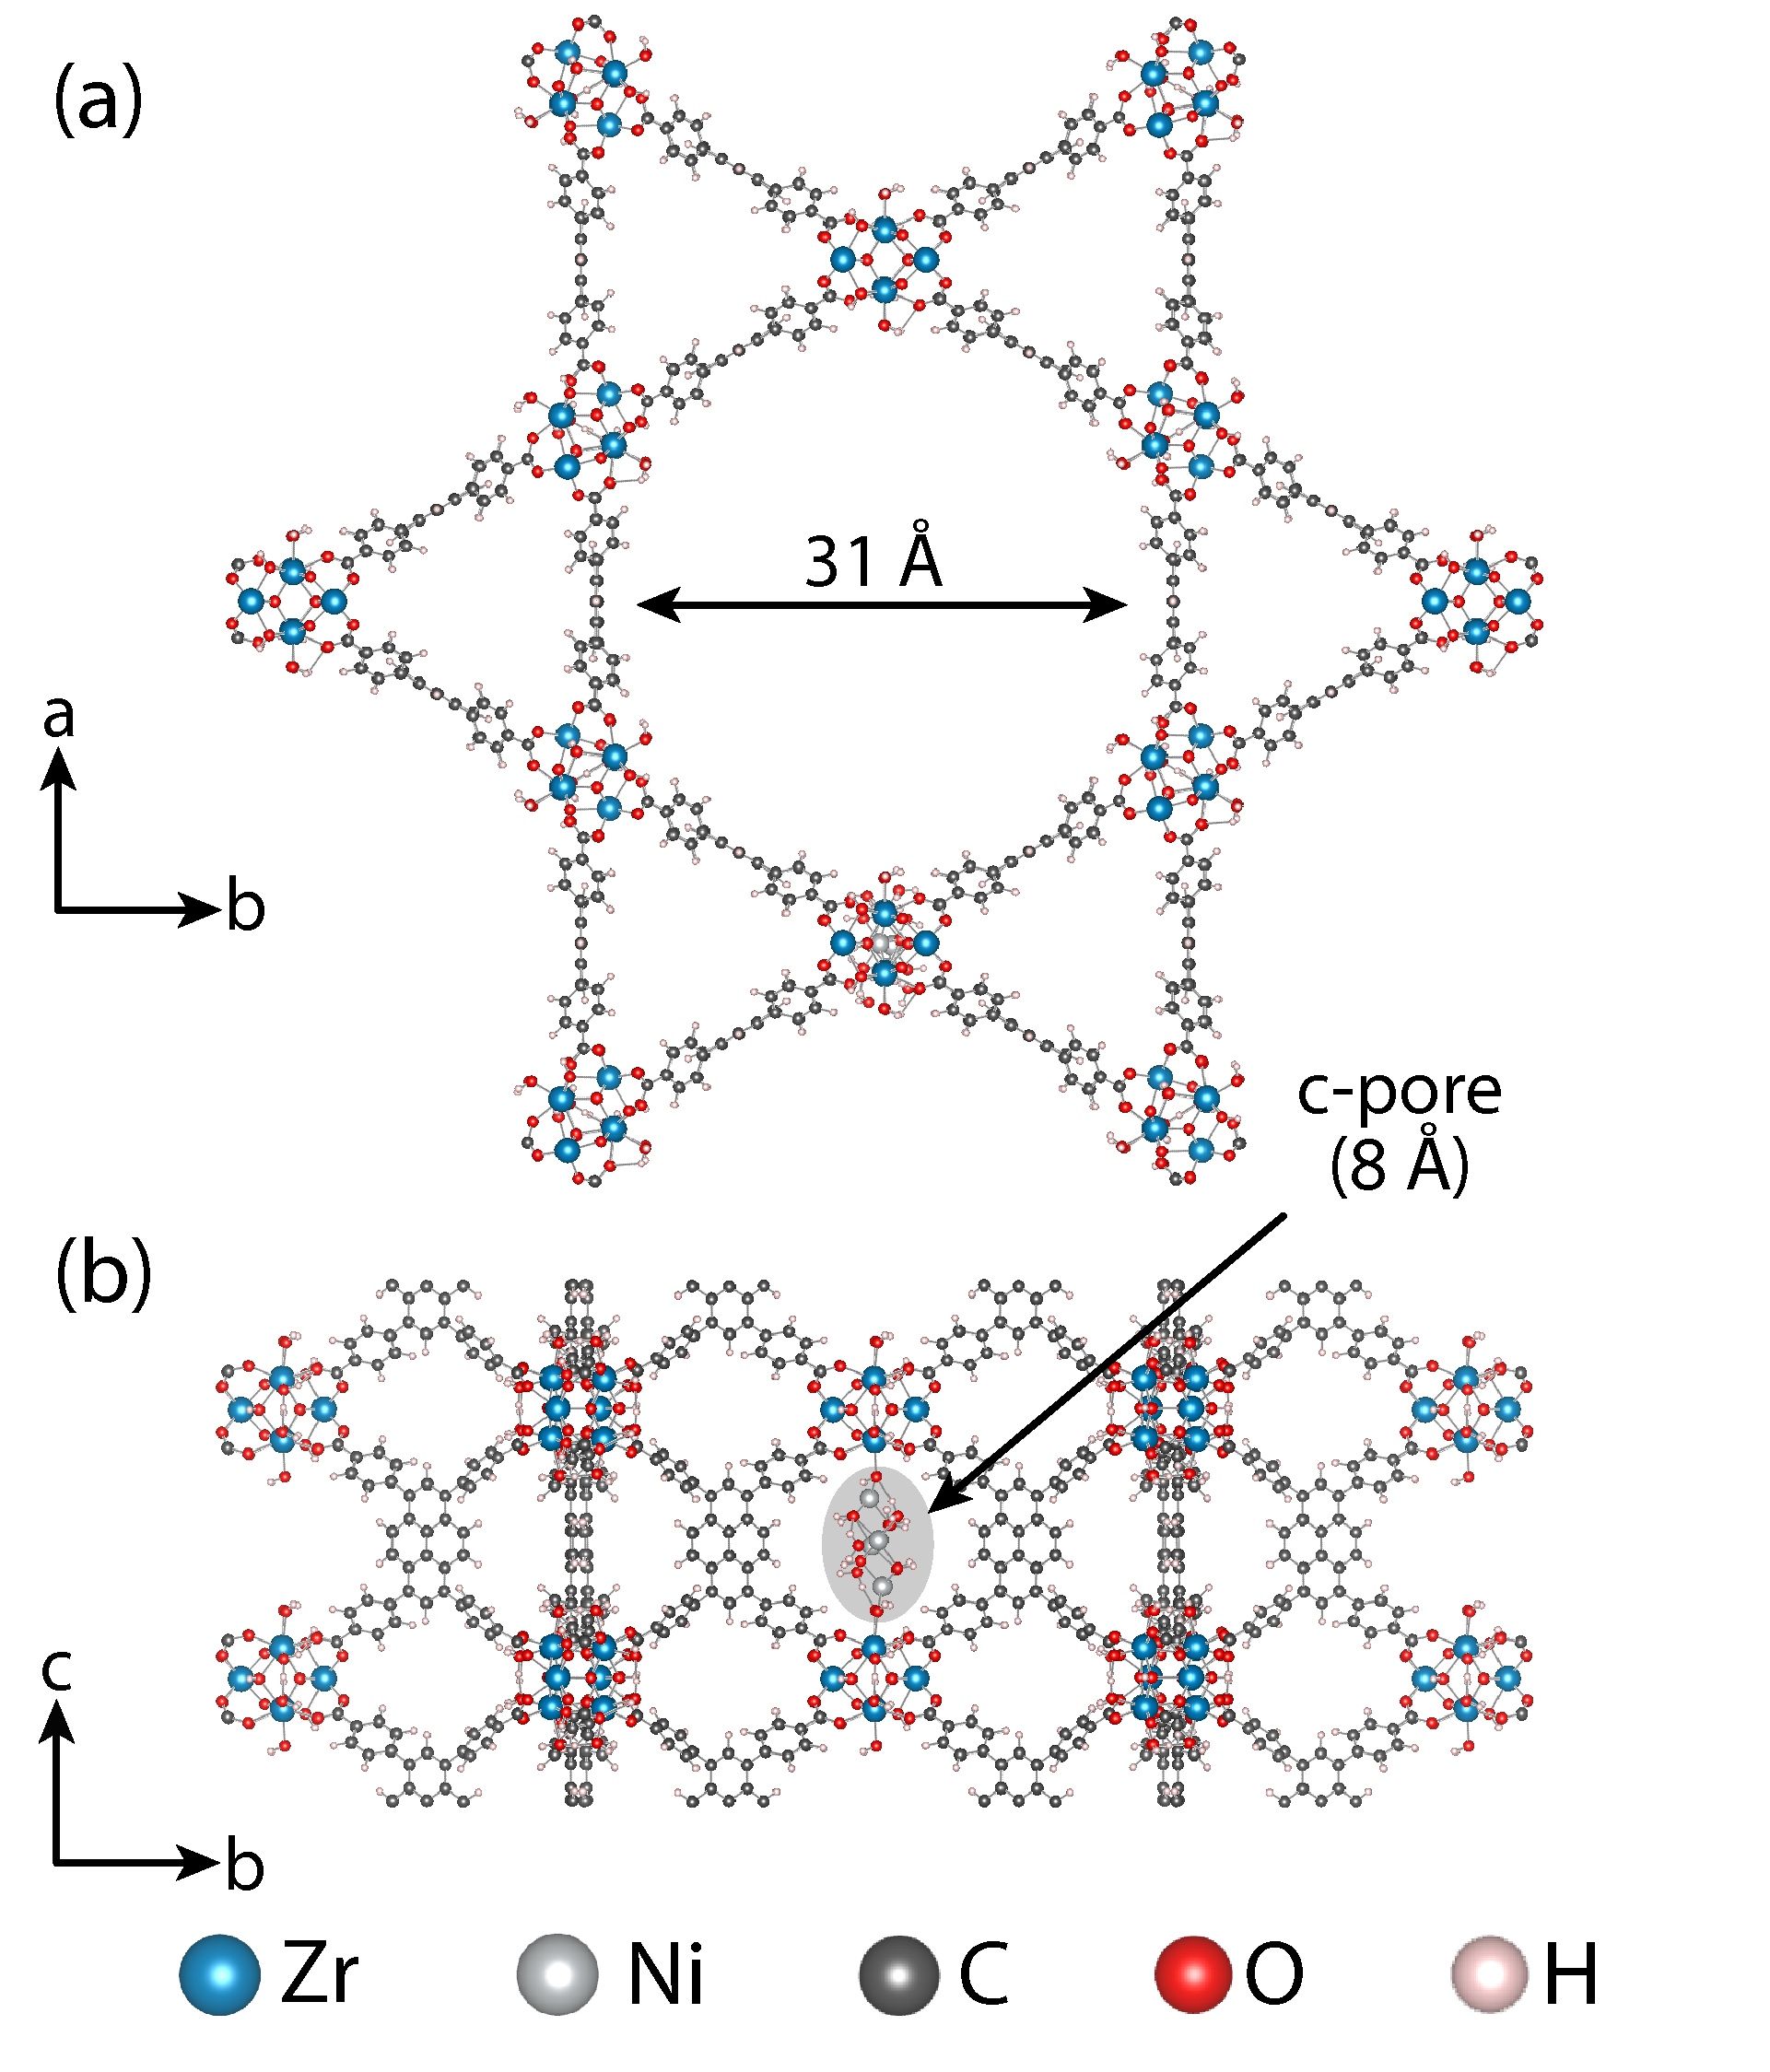
\includegraphics[width=3.0in]{zi-images/00-General-Graphics/2022-figure-MOF-schematic.png}
    \caption{
    The structure of NU-1000 shown along the (a) c-axis and the (b) a-axis with the location of the \ce{Ni} metal cluster highlighted by the gray oval. The metal cluster is located within the 8~{\AA} pore of Ni-NU-1000. The diameters of the hexagonal (31~{\AA}) and triangular (10~{\AA}) channels are also indicated.
    }
    \label{fig:Ni-MOF-model}
\end{figure}

\subsection{Pair Distribution Function (PDF) Analysis}
Powder X-ray diffraction (XRD) and total scattering data suitable for PDF analysis are collected on Ni-NU-1000 catalysts at 50 \degree C in \ce{H2}, as described in a prior publication.\cite{PlateroPrats2017} The PDF provides structural information such as the distribution of interatomic distances in the Ni-NU-1000 catalysts and also reflects the \ce{Ni} coordination number and asymmetry in the \ce{Ni} coordination environment. PDFs represent the local structure as a histogram of atom-atom distances weighted by the scattering power of the atoms involved. Of interest are the \ce{Ni{\Compactcdots}Ni} and \ce{Ni-O} distances within the cluster and the \ce{Ni{\Compactcdots}Zr} distance between the cluster and NU-1000. In this notation, atom pairs not directly bonded to each other are denoted with ``${\Compactcdots}$". Given the lower scattering contribution from the \ce{O} atoms compared to \ce{Ni} atoms, \ce{O{\Compactcdots}O} pairs have very low contribution to the measured data and are not calculated. PDFs are used to derive d-PDFs by subtracting the PDF measured for NU-1000 from the PDF measured for Ni-NU-1000, to isolate the atom-atom distances that define the \ce{Ni} cluster and its interaction with NU-1000 support. The PDFs for the structures are calculated using the PDFgui software.\cite{Farrow2007}

\subsection{Computational Details}

\subsubsection{Catalyst Structure Models}

Modeling is carried out to provide molecular level insight into the ligand environment of Ni-NU-1000. NU-1000 crystallizes in the P6/mmm space group, with unit cell models employing DFT-optimized parameters of $a=b=40.611$ {\AA}, $c=15.990$ {\AA}, $\alpha=\beta=\ang{90}$, and $\gamma=\ang{60}$. Following prior work,\cite{Ye2017} \ce{Ni4} clusters are used to model the \ce{Ni} catalyst. Clusters comprising fewer than four \ce{Ni} ions were also evaluated, but gave poor agreement with the experimental d-PDF (see Supporting Information Section S3). \ce{Ni4} clusters span the 8 {\AA} pores of NU-1000, connecting two adjacent nodes (Figure~\ref{fig:Ni-MOF-model}b) by replacing a proton on each node.\cite{Ye2017} 

To provide molecular-level insight into the types of ligand environments that could lead to the experimentally observed d-PDFs, 854 different ligand environments are considered. These ligand environments include \ce{OH}, \ce{H2O}, \ce{H}, and \ce{O}, and have stoichiometries of \ce{Ni_4O_xH_y}. Four example structures are shown in Figure~\ref{fig:Ni-MOF-structures}. The full library of structures considered in this work can be accessed on GitHub.\cite{GitHub-Ni4Project} The \ce{Ni-O} coordination numbers are calculated according to geometric criteria (distance and orientation) as discussed in Supporting Information Section S1.7. 

\begin{figure}
    \centering
    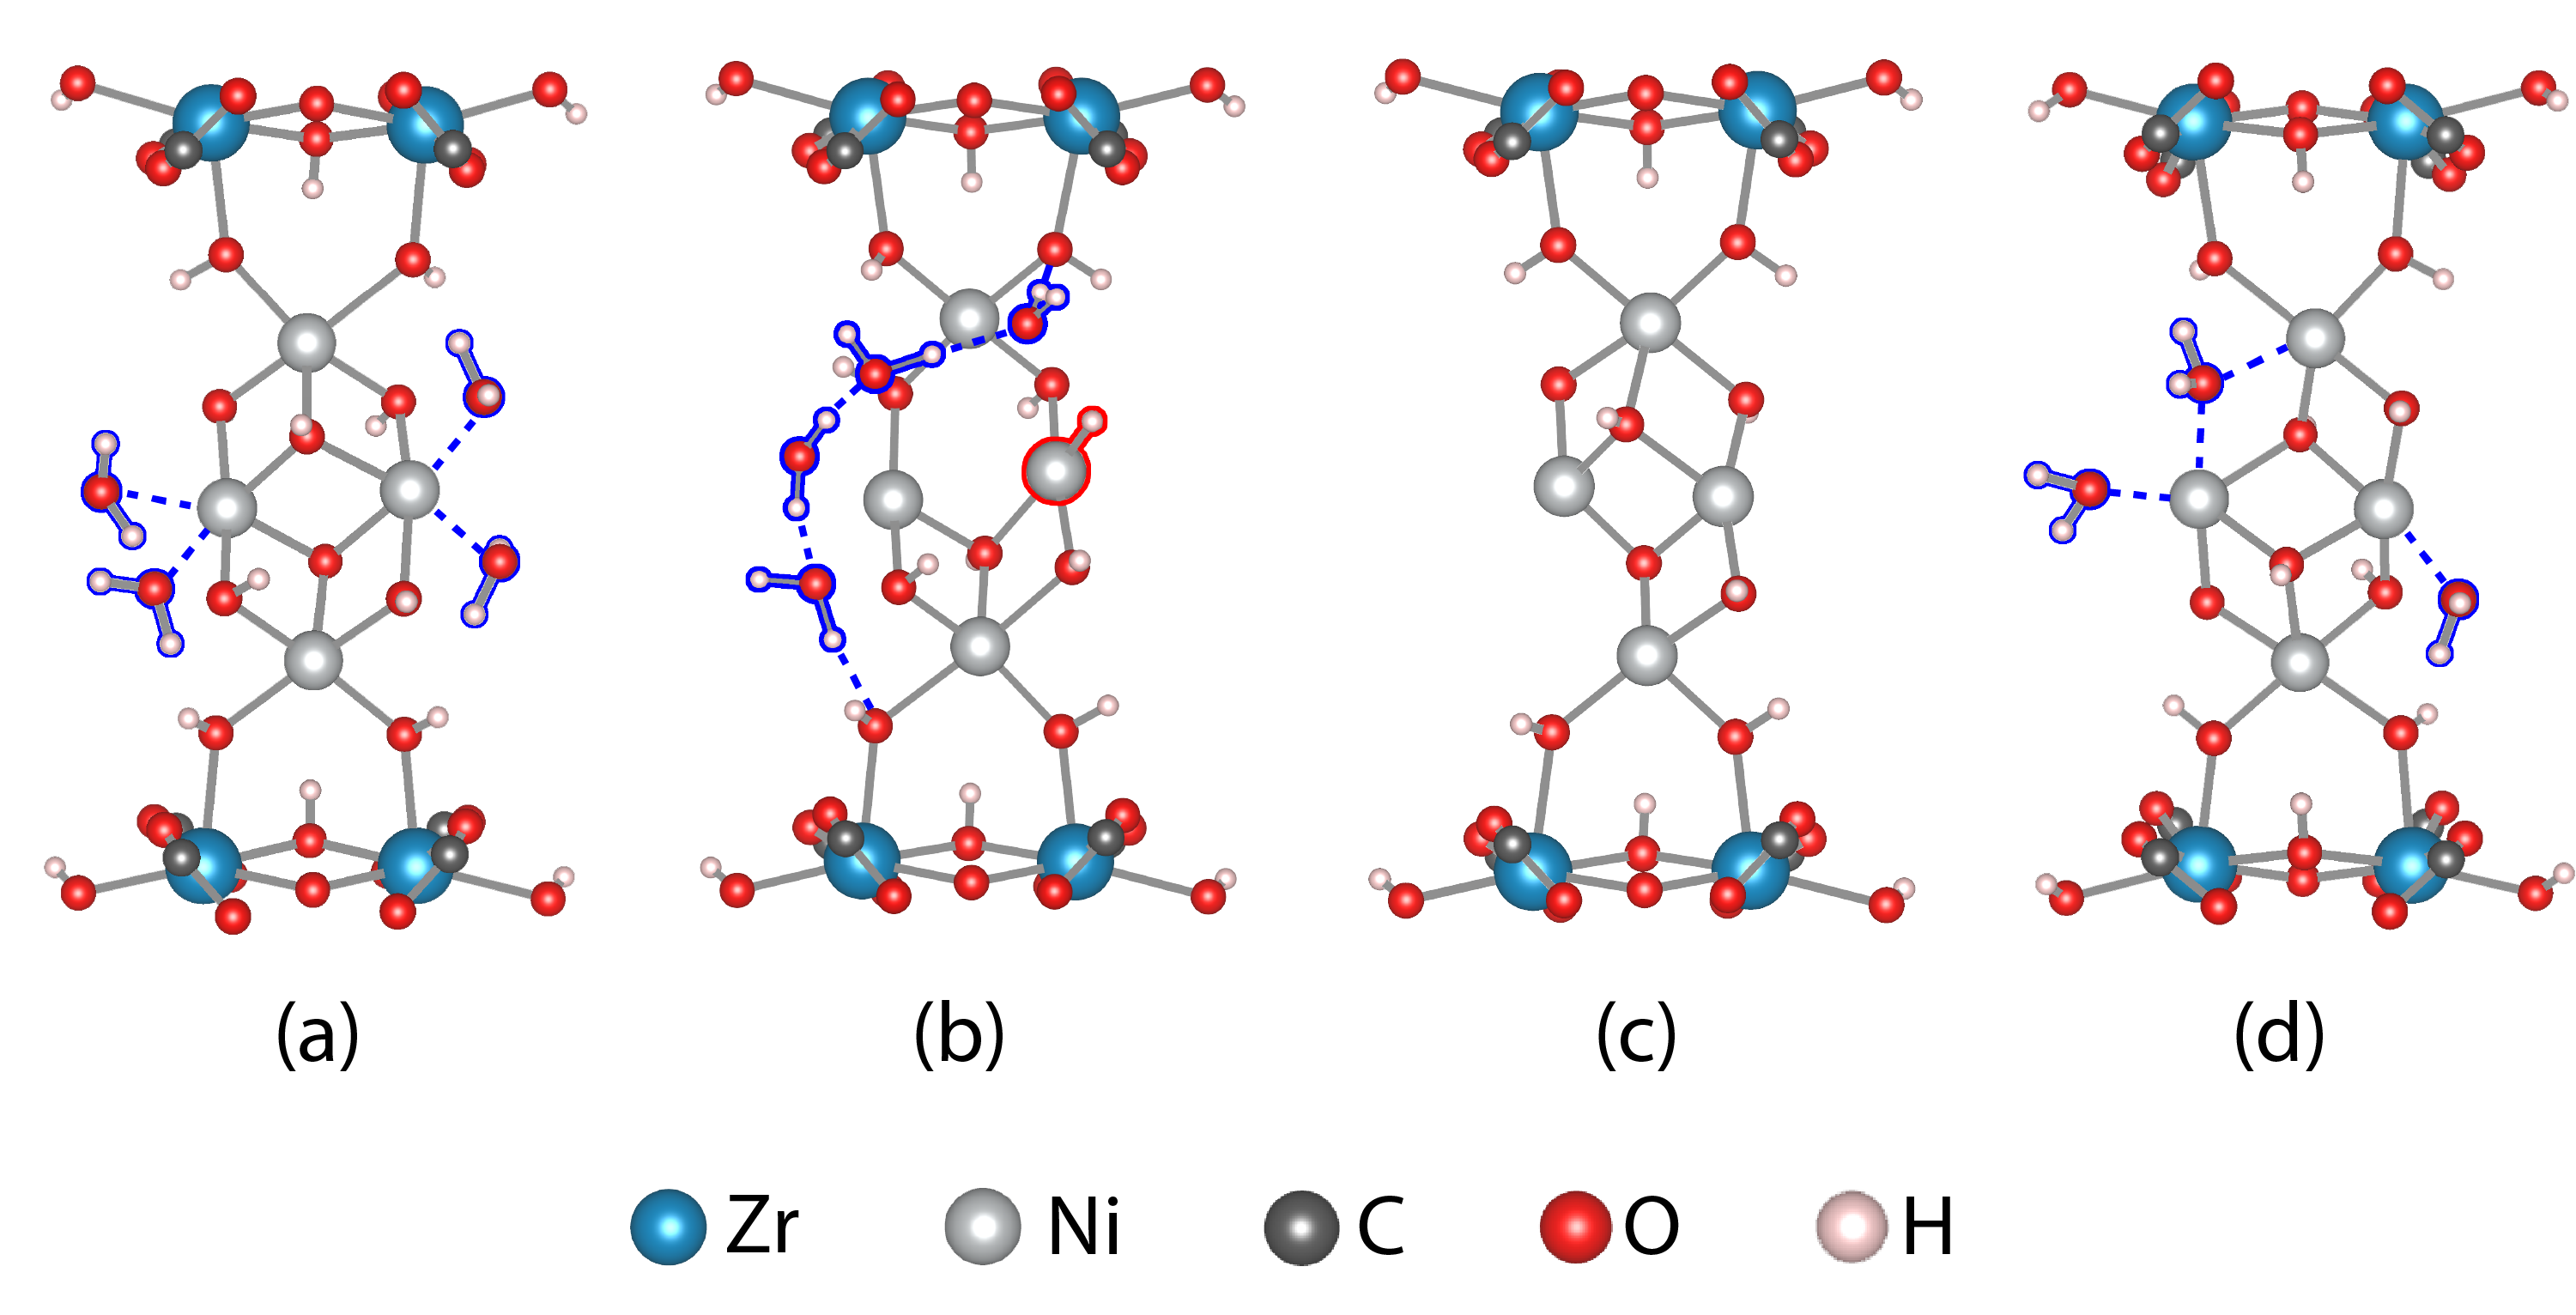
\includegraphics[width=5.0in]{zi-images/00-General-Graphics/2022-figure-clusters-3xstructures.png}
    \caption{
    Some of the \ce{Ni_4O_xH_y} clusters evaluated in this work. (a) \ce{Ni4(OH)6.4H2O} (green), (b) \ce{Ni4(OH)5(H).4H2O} (blue), (c) \ce{Ni4(OH)4(O)} (yellow), and (d) \ce{Ni4(OH)4(O).3H2O} (maroon). Colors in parentheses are the same as for Figures~\ref{fig:phase_diagram_Ni} and \ref{fig:Ni-structure-diagram}. The NU-1000 structure is excluded from the pictures for clarity, except for the \ce{Zr} ions where the clusters are attached. The atom color key is indicated in the figure. \ce{H2O} molecules and ligands are outlined in blue, and \ce{Ni-H} ligands are outlined in red.
    }
    \label{fig:Ni-MOF-structures}
\end{figure}

\subsubsection{\textit{ab initio} Thermodynamics Modeling}

\textit{ab initio} thermodynamic analysis\cite{Reuter2003, Reuter2004, Grundner2015, Paolucci2016, Li2016, Getman2008, Mandal2020, Zuo2016, Tang2019} is used to determine the thermodynamically stable structures as functions of chemical potential (which can be related to gas phase temperature and partial pressure using an equation of state; see Supporting Information Section S1.3). We specifically consider chemical potentials of \ce{H2} (g) ($\mu_{\ce{H2}}$) and \ce{H2O} (g) ($\mu_{\ce{H2O}}$). \ce{H2} (g) is chosen since experimental d-PDFs were collected under hydrogenation conditions. \ce{H2O} (g) is chosen since we find hydrogen atom binding on the cluster often occurs on hydroxyl ligands, forming \ce{H2O} ligands, which can then desorb. \ce{H2O} (g) is hence a convenient oxygen reference (see Figure~S1). Cluster free energies are calculated as:
\begin{equation}
    \begin{split}
        \Delta F^{(2)}(V,T,\mu_{\text{H}},\mu_{\text{O}},N_{\text{Ni}})  
        & = \Delta F(V,T,N_{\text{H}},N_{\text{O}},N_{\text{Ni}}) - (\mu_{\text{H}})(\Delta N_{\text{H}}) \\
        & - (\mu_{\text{O}})(\Delta N_{\text{O}})  \\ 
    \end{split}
    \label{eq:free-energy-trans}
\end{equation}
where $F^{(2)}$ is the the second Legendre transform of the Helmholtz free energy (i.e., of $N_{\ce{H}}$ and $N_{\ce{O}}$ to $\mu_{\ce{H}}$ and $\mu_{\ce{O}}$),\cite{Alberty1997} $V$ is volume, $T$ is temperature, $\mu$ is chemical potential, and $N$ is number, i.e., of \ce{O} and \ce{H} atoms within the cluster. Here $\mu_{\ce{H}} = \frac{1}{2} \mu_{\ce{H}_2}$, and $\mu_{\text{O}} = \mu_{\ce{H2O}} - 2\mu_{\ce{H}}$. $F = E^\text{elec} + E^\text{ZP} + F^\text{vib}$, where $E^\text{elec}$ is the electronic energy calculated with DFT, $E^\text{ZP}$ is the zero point vibrational energy, and $F^\text{vib}$ is the temperature dependent vibrational free energy. The $\Delta$'s in Eq.~\ref{eq:free-energy-trans} indicate quantities taken relative to a reference structure; the reference structure used in this work is the \ce{Ni4(OH)6.4H2O} structure shown in Figure~\ref{fig:Ni-MOF-structures}a, which comprises \ce{OH} and \ce{H2O} ligands (outlined in blue in Figure~\ref{fig:Ni-MOF-structures}).

\subsubsection{Density Functional Theory Calculations}
Electronic energies are calculated using the CP2K software package\cite{Hutter2014} using the PBE exchange and correlation functional\cite{Perdew1996}, damped D3 dispersion corrections,\cite{Grimme2010} the DZVP-MOLOPT basis set,\cite{VandeVondele2007} and Goedecker pseudopotentials.\cite{Goedecker1996} Plane waves are simulated up to 360 Ry. As a single \ce{Ni} ion can adopt singlet or triplet spin states, we evaluate singlet, triplet, quintet, septet, and nonet states for the \ce{Ni4} clusters, following prior work.\cite{Shabbir2020, Ye2017, Bernales2016} The unrestricted Kohn-Sham (UKS) method is employed given the open shell nature of the system. Spin states exhibiting spin contamination are not considered in \textit{ab initio} thermodynamic analysis. Details about how spin contamination is determined and the criteria used to keep or discard structures is provided in Supporting Information Section S1.6. Electronic energies are obtained from geometry relaxations where all atoms in the periodic unit cell are allowed to relax. $E^\text{ZP}$ and $F^\text{vib}$ are calculated from the calculated vibrational modes. Details about how the vibrational modes, $E^\text{ZP}$, and $F^\text{vib}$ are calculated are provided in Supporting Information Section S1.4. Vibrational modes are only calculated for structures within 100 kJ/mol of the lowest electronic-energy cluster at each unique composition to decrease computational expense. Details about how $E_{\text{H}_2}$ and $E_{\text{H}_2\text{O}}$ are calculated and sample CP2K input files for all types of DFT calculations carried out in this work are provided in Supporting Information Sections S1.8, S1.9, and S.10. 

\section{Results}
%%%%%%%%%%%%%%%%%%%%%%%%%%%%%%%%%%%%%%%%%%%%%%%%%%%%%%%%%%%%%%%%%%%%%
%% Results 
%%%%%%%%%%%%%%%%%%%%%%%%%%%%%%%%%%%%%%%%%%%%%%%%%%%%%%%%%%%%%%%%%%%%%

% d-PDF Diagram
\begin{figure}
    \centering
    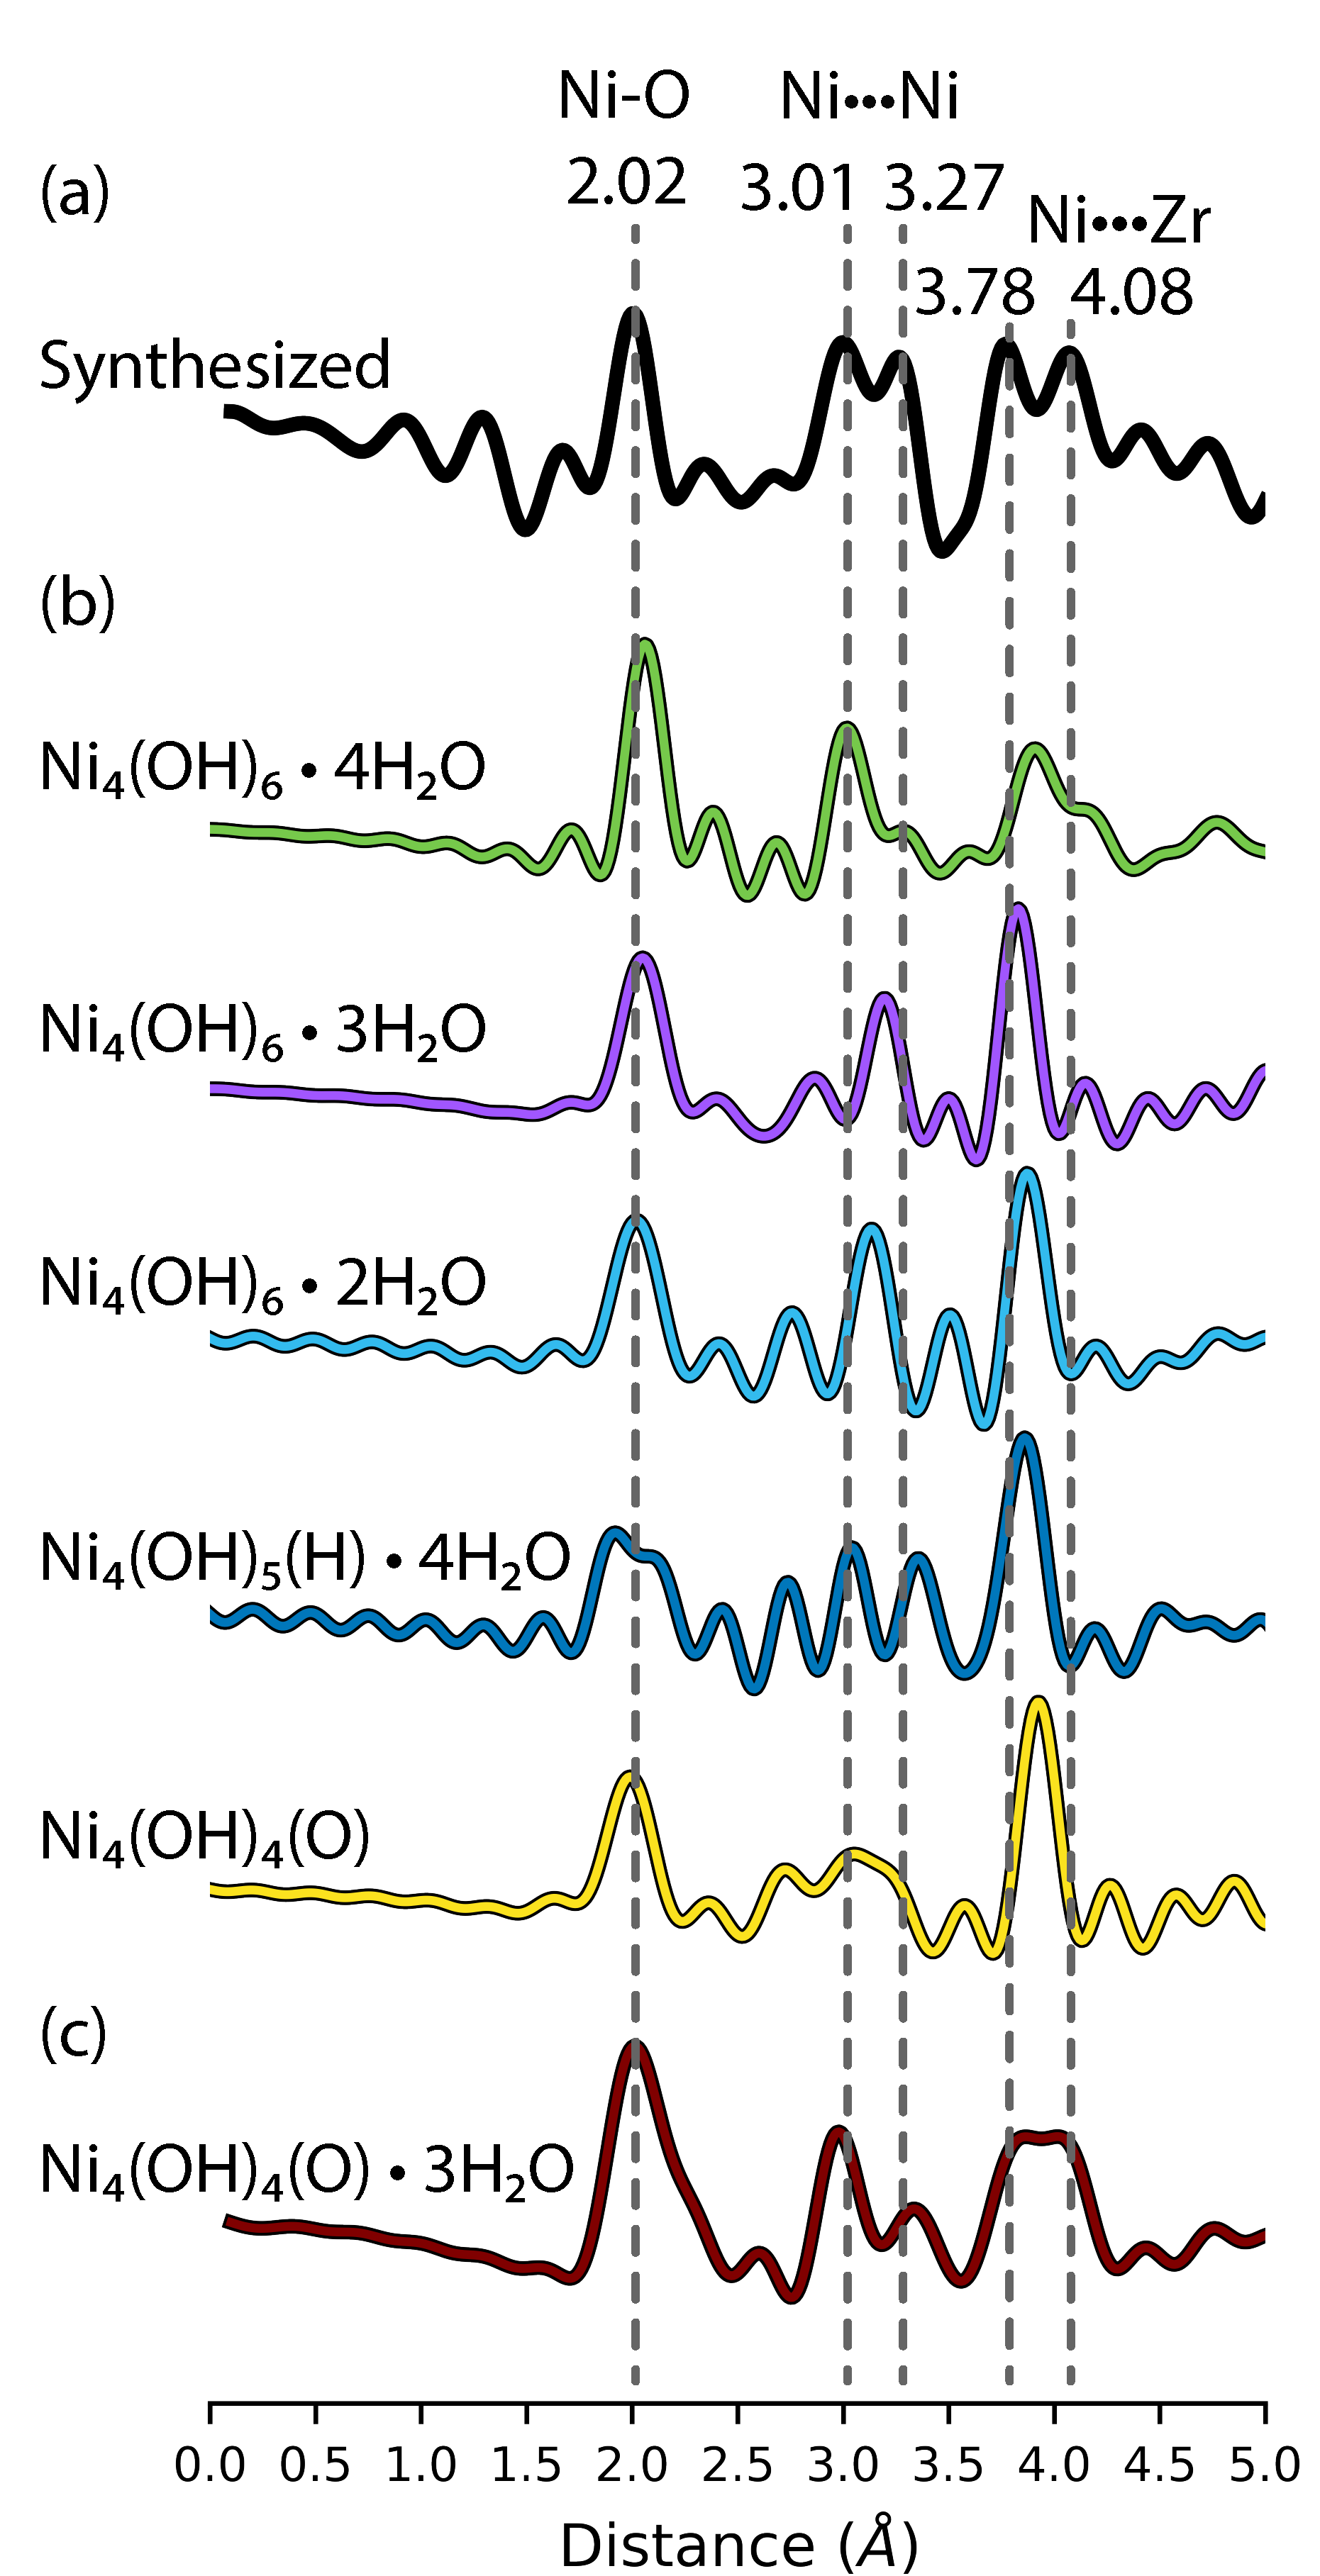
\includegraphics{zi-images/01-Ni-Graphics/2021-MAIN-single-dPDF.png}
    \caption{
    d-PDFs for (a) the synthesized structure, (b) the simulated structures representing thermodynamic minima with \ce{Ni-O} coordination numbers $\ge$ 4, (c) the simulated structures that give the best agreement with the synthesized structure, and (d) the Boltzmann weighted d-PDF. Structure labels and colors for the simulated structures are the same as in the text and in Figures~\ref{fig:phase_diagram_Ni} and \ref{fig:Ni-structure-diagram}. Gray dotted lines indicate key distances observed for the synthesized structure, which are also annotated on the figure. A peak labeled with $\ast$ indicates a \ce{Ni-O} peak, the $\ddagger$ indicates a \ce{Ni{\Compactcdots}Ni} peak, and the $\times$ indicates a \ce{Ni{\Compactcdots}Zr} peak.
    }
    \label{fig:dPDFs-graphic}
\end{figure}

The d-PDF for the synthesized Ni-NU-1000 catalyst is shown in Figure~\ref{fig:dPDFs-graphic}a.\cite{PlateroPrats2017} Key peaks are the single peak at 2.02 {\AA}, split peaks at 3.01 {\AA} and 3.27 {\AA}, and split peaks at 3.78 {\AA} and 4.08 {\AA}, which correspond to \ce{Ni-O}, \ce{Ni{\Compactcdots}Ni}, and \ce{Ni{\Compactcdots}Zr} distances, respectively. Prior work indicates that the average \ce{Ni-O} coordination number is $\sim$5.\cite{PlateroPrats2017} 

The most stable structures from modeling are presented in Figure~\ref{fig:phase_diagram_Ni}. In this phase diagram, the different colored regions correspond to different structures, which are depicted in Figure~\ref{fig:Ni-structure-diagram}a. Each structure is annotated with its \ce{Ni-O} coordination number; ranges of $\mu_{\ce{H2}}$ and $\mu_{\ce{H2O}}$ are selected such that coordination numbers $\sim$5 are centered in order to match experimental findings. Expansion of the phase diagram to higher and lower values of $\mu_{\text{H}_2\text{O}}$ and $\mu_{\text{H}_2}$ does not reveal any additional structures or higher coordination numbers (see Supporting Information Section S4). The \ce{Ni4(OH)6.2H2O}, \ce{Ni4(OH)6.3H2O}, and \ce{Ni4(OH)6.4H2O} structures (represented by the cyan, purple, and green regions on the phase diagram) give \ce{Ni-O} coordination numbers of 5.0, 5.25, and 5.5, which are in line with the experimentally observed value of $\sim$5. These structures comprise significant \ce{OH} and \ce{H2O} ligands and no \ce{O} or \ce{H} ligands (Figure~\ref{fig:Ni-structure-diagram}a). They reside on the phase diagram at higher (more positive) values of $\mu_{\text{H}_2\text{O}}$ and lower (more negative) values of $\mu_{\text{H}_2}$. As the experimental d-PDF was obtained under hydrogenation conditions, this suggests that the \ce{H2O} is coming from NU-1000. Similar \ce{H2O} storage properties have been observed in MOF-303\cite{Hanikel2021} and MOF-801.\cite{Kim2017} The vertical dotted line in Figure~\ref{fig:phase_diagram_Ni} indicates values of $\mu_{\ce{H2}}$ used during collection of the experimental d-PDF. The \ce{Ni4(OH)6.3H2O} (purple) and \ce{Ni4(OH)5(H).4H2O} (blue) structures fall along this line. The \ce{Ni4(OH)5(H).4H2O} (blue) structure has a slightly lower coordination number of 4.25. It also comprises significant \ce{OH} and \ce{H2O} content and includes a \ce{H} ligand. 

% Phase Diagram
\begin{figure}[H]
    \centering
    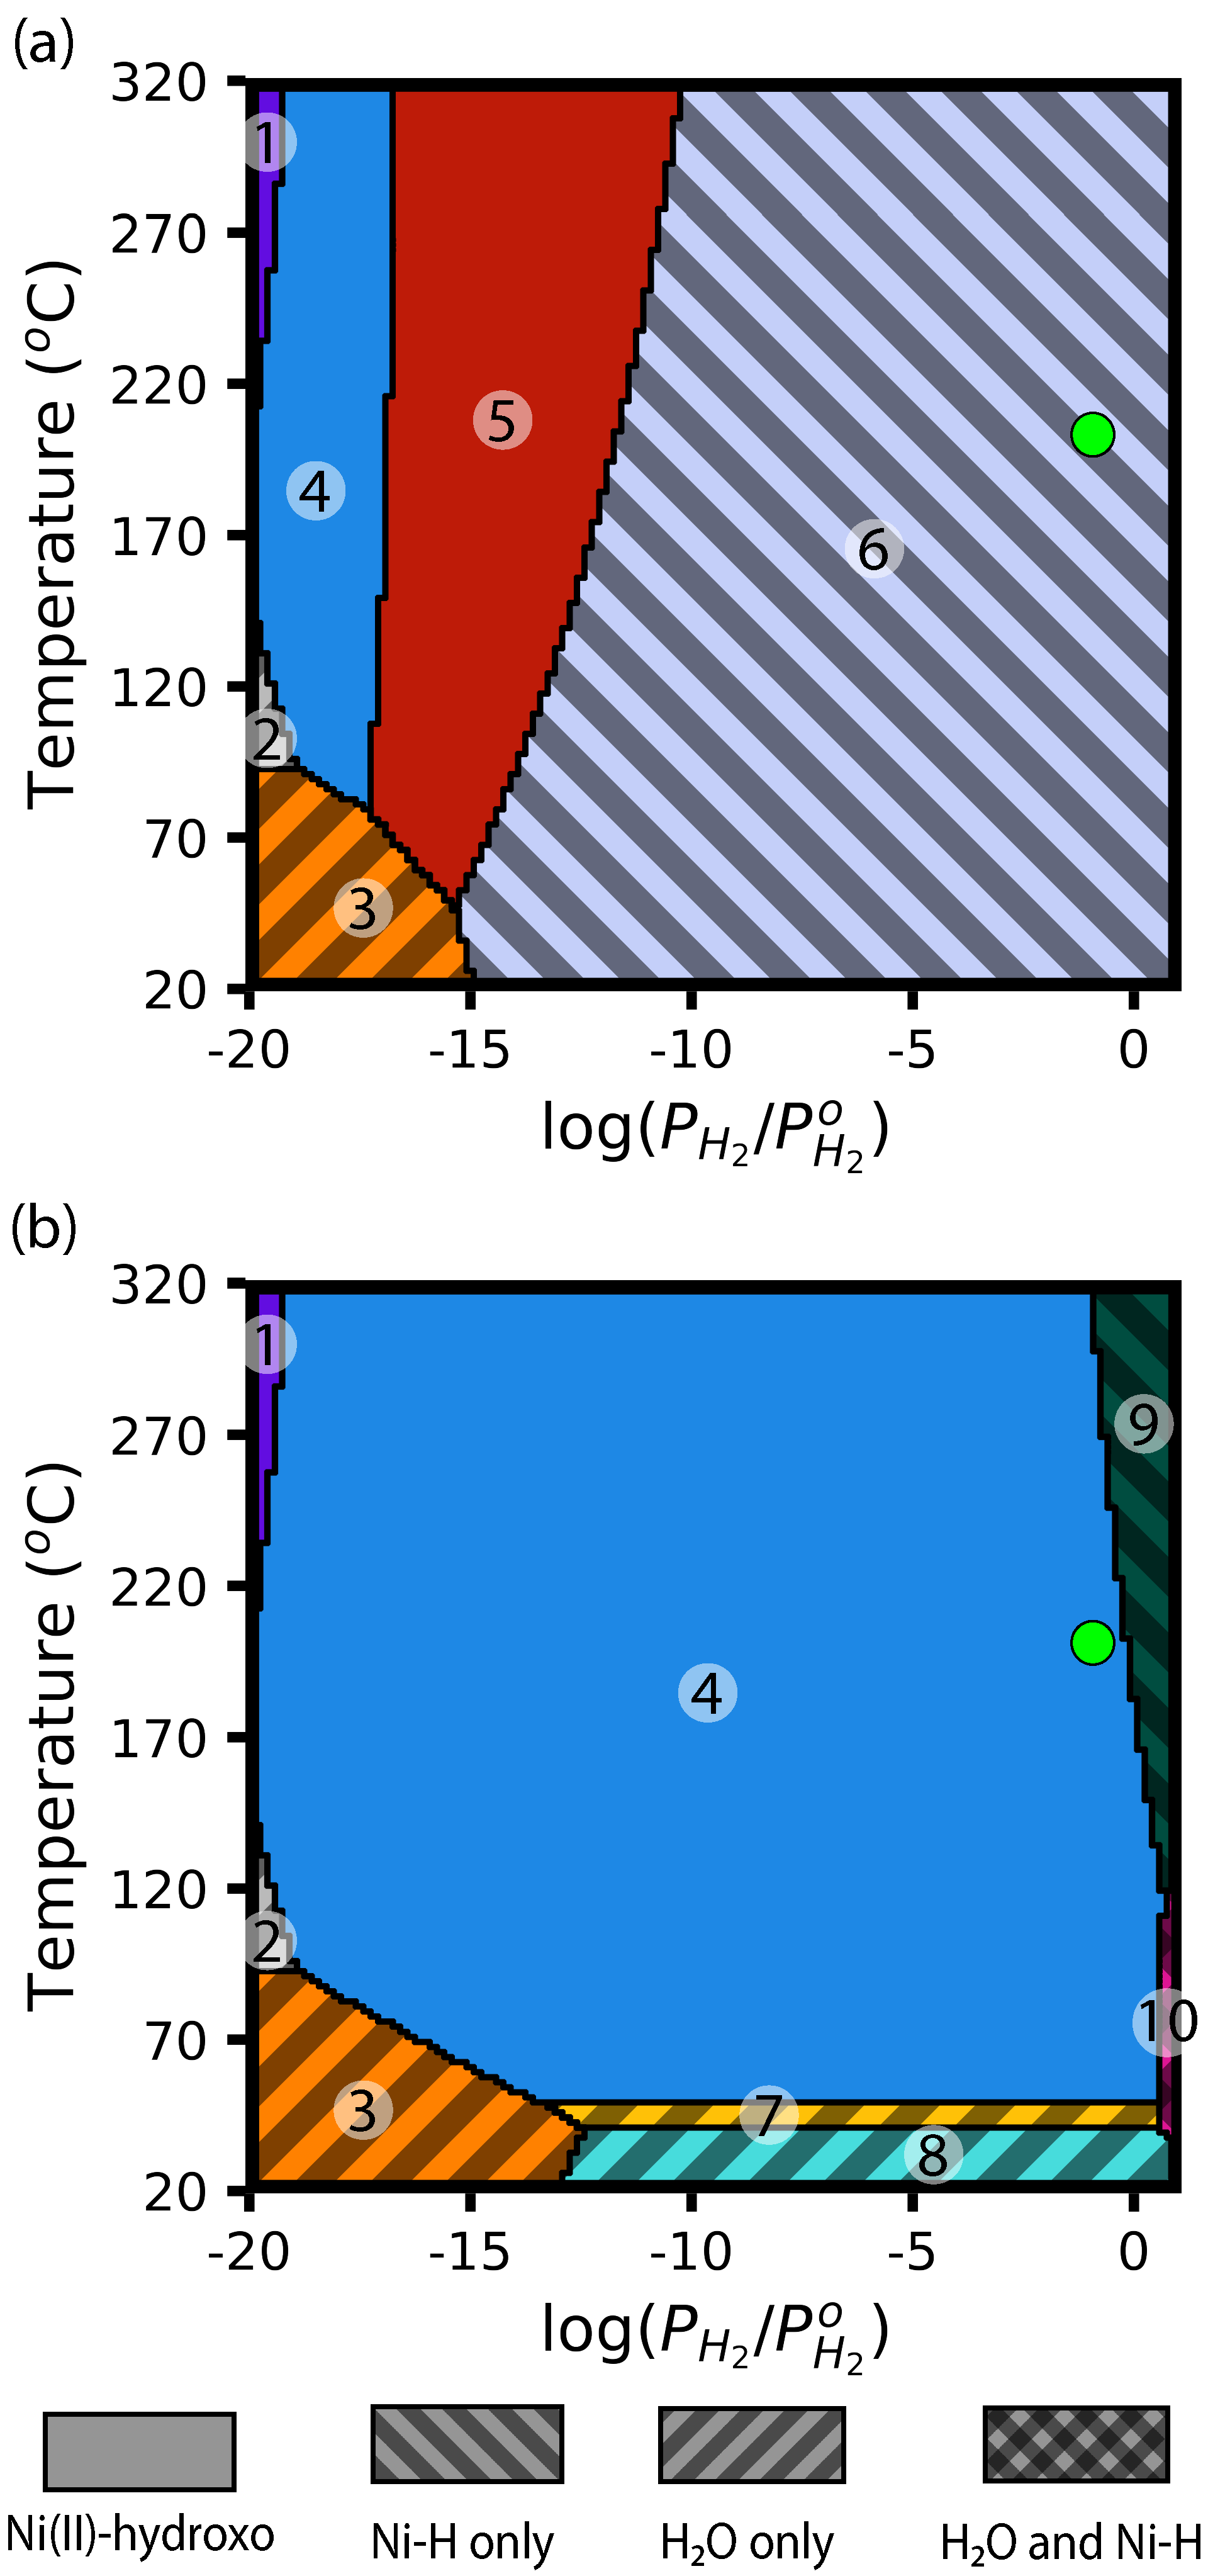
\includegraphics{zi-images/01-Ni-Graphics/2021-MAIN-phase-diagram-combined.png}
    \caption{
    Calculated phase diagram for the \ce{Ni4} cluster presented as a function of $\Delta \mu_{\ce{H2}}$ and $\Delta \mu_{\ce{H2O}}$, where the $\Delta$'s indicate the values are referenced to the 0~K values (derivation provided in Supporting Information Section S1.5). The different colored regions indicate different structures and follow the same key as in Figures~\ref{fig:dPDFs-graphic} and \ref{fig:Ni-structure-diagram}. The numbers indicate the \ce{Ni-O} coordination number. The hash patterns indicate the types of ligand environments and follow the key in the figure. The vertical dashed line indicates the value of $\Delta \mu_{\text{H}_2}$ corresponding to the conditions where the experimental d-PDF was collected (\ce{H2} in 3.5\% in \ce{He} at 50 \degree C and ambient pressure).\cite{PlateroPrats2016} As \ce{H2O} was not added in experiments, values of $\Delta \mu_{\ce{H2O}}$ are chosen such that the \ce{Ni-O} coordination number matches the experimentally observed value of $\sim$5 (e.g., $\Delta \mu_{\ce{H2O}} > \sim -40$ along the vertical dashed line). Structures with \ce{Ni-O} coordination numbers $\ge$ 4.0 are \ce{Ni4(OH)4(O)} (yellow; 4.0), \ce{Ni4(OH)5(H).4H2O} (blue; 4.25), \ce{Ni4(OH)6.2H2O} (cyan; 5.0), \ce{Ni4(OH)6.3H2O} (purple; 5.25), and \ce{Ni4(OH)6.4H2O} (green; 5.5).
    }
    \label{fig:phase_diagram_Ni}
\end{figure}  

% Structure Diagram
\begin{figure}
    \centering
    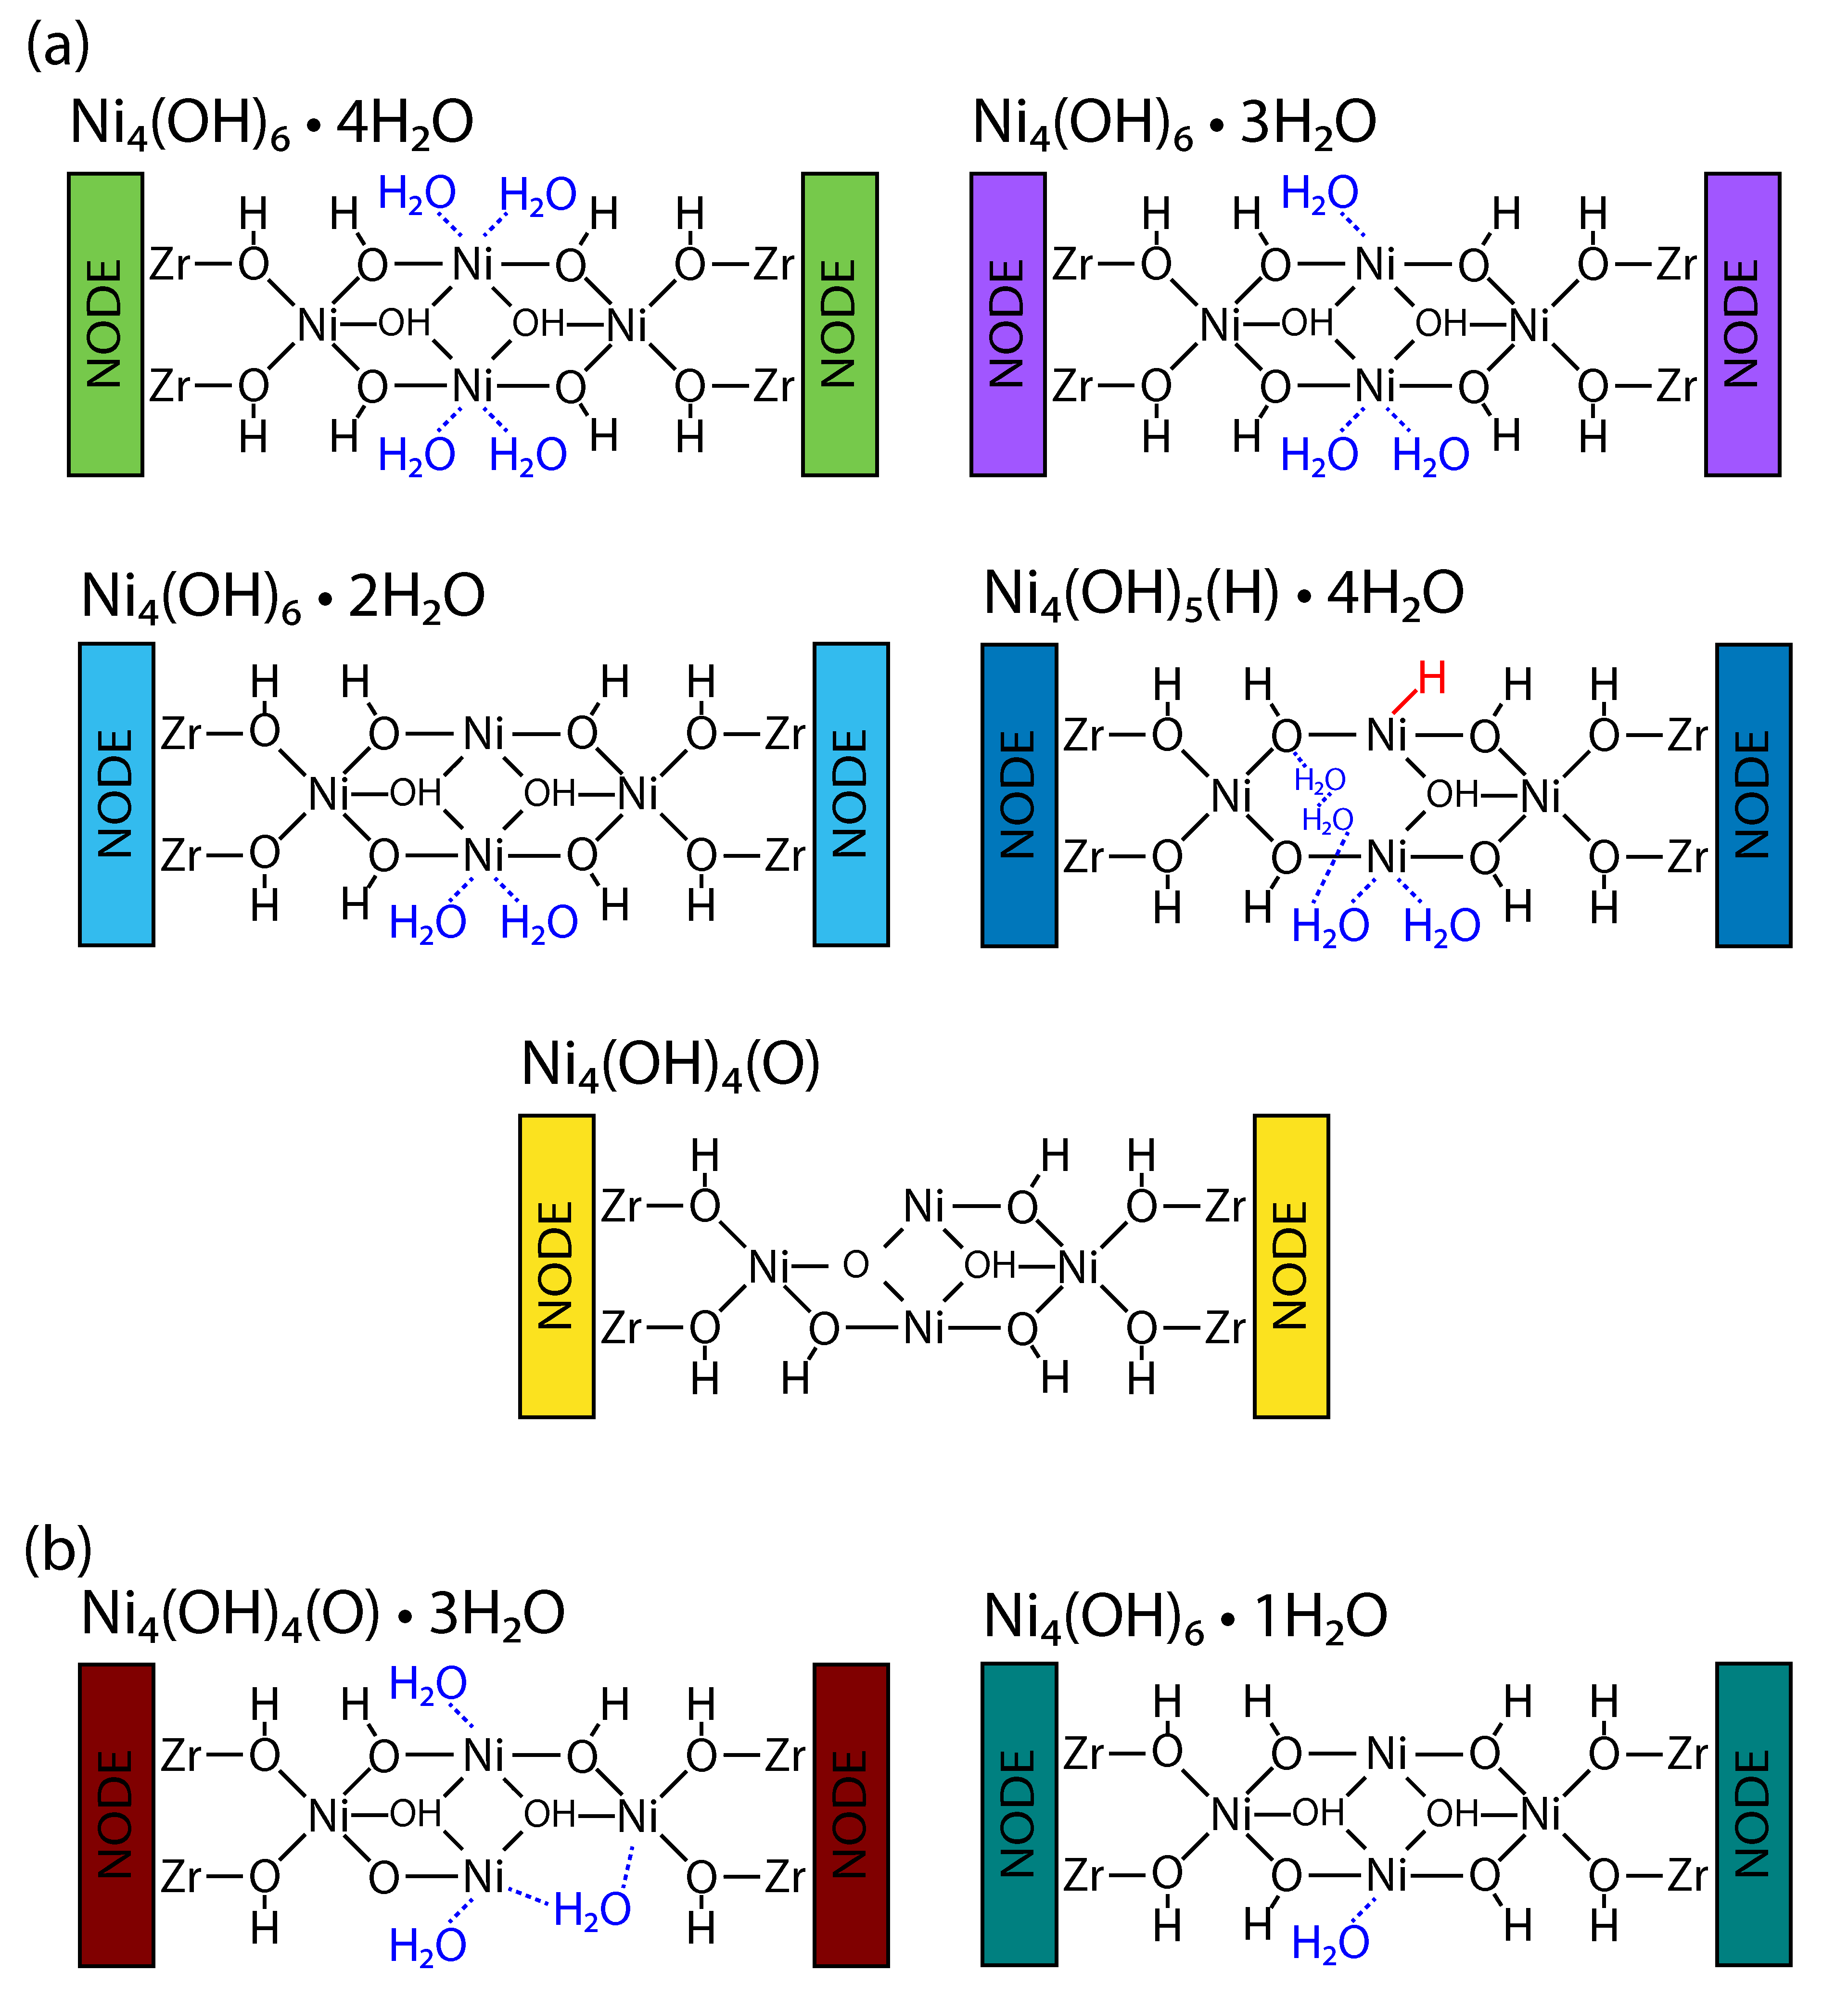
\includegraphics[width=0.75\textwidth]{zi-images/01-Ni-Graphics/2021-MAIN-structure-diagram.png}
    \caption{
    Depictions of (a) structures from Figure~\ref{fig:phase_diagram_Ni} with \ce{Ni-O} coordination numbers $\ge$ 4 and (b) the structures that exhibit d-PDFs that give the best agreement with that of the synthesized structure. The color scheme is the same as in Figures~\ref{fig:dPDFs-graphic} and \ref{fig:phase_diagram_Ni}. \ce{H2O} molecules and ligands are indicated with blue text, and \ce{Ni} hydrides are indicated with red text for emphasis. Color code: Part a: Top row: green (left), purple (right). Second row: cyan (left), blue (right). Third row: yellow. Part b: maroon (left), teal (right).  
    }
    \label{fig:Ni-structure-diagram}
\end{figure}

To compare with experiment, d-PDFs for all structures on the phase diagram with \ce{Ni-O} coordination numbers $\ge$ 4 are shown in Figure~\ref{fig:dPDFs-graphic}b. We seek structures that give good agreement with the \ce{Ni-O} and \ce{Ni{\Compactcdots}Ni} peaks seen in the experimental d-PDF, as matching these peak positions provides insights into the ligand environments of the \ce{Ni} ions. \ce{Ni-O} peaks in general agree well with experiment, except for \ce{Ni4(OH)5(H).4H2O} (blue), which exhibits split peaks instead of a single peak. One rationale for the split peaks is asymmetry of the ligand environments of the different \ce{Ni} ions in the cluster. From Figure~\ref{fig:Ni-structure-diagram}a, the different \ce{Ni} ions in the \ce{Ni4(OH)5(H).4H2O} (blue) structure indeed exhibit different ligand environments, with one \ce{Ni} ion comprising four \ce{OH} ligands, one comprising five \ce{OH} ligands, one comprising \ce{OH} and \ce{H} ligands, and another comprising \ce{OH} and \ce{H2O} ligands. Interestingly, the \ce{Ni} ion that connects to \ce{OH} and \ce{H2O} ligands also connects to a hydrogen bonded chain of \ce{H2O} molecules. In the remainder of the structures, which exhibit a single \ce{Ni-O} peak (in agreement with experiment), all \ce{Ni} ions connect to \ce{OH} and \ce{H2O} ions. These results suggest that \ce{Ni} ions in \ce{Ni}-NU-1000 catalysts comprise \ce{OH} and \ce{H2O} ligands, but not \ce{H} ligands. 

There is less agreement between simulations and experiments for the \ce{Ni{\Compactcdots}Ni} peaks in the d-PDFs in Figures~\ref{fig:dPDFs-graphic}a and b. In the experimental d-PDF (Figure~\ref{fig:dPDFs-graphic}a), these peaks are split. In contrast to this, most of the simulated structures in Figure~\ref{fig:dPDFs-graphic}b exhibit a single \ce{Ni{\Compactcdots}Ni} peak. The exceptions are \ce{Ni4(OH)5(H).4H2O} (blue) (Figures~\ref{fig:Ni-MOF-structures}b and~\ref{fig:Ni-structure-diagram}a), \ce{Ni4(OH)6.2H2O} (cyan) (Figure~\ref{fig:Ni-structure-diagram}a), and \ce{Ni4(OH)4(O)} (yellow) (Figures~\ref{fig:Ni-MOF-structures}c and~\ref{fig:Ni-structure-diagram}a). \ce{Ni4(OH)5(H).4H2O} (blue) exhibits three \ce{Ni{\Compactcdots}Ni} peaks due to the highly asymmetric ligand environment, which disagrees with experimental observation. In contrast, \ce{Ni4(OH)6.2H2O} (cyan) and \ce{Ni4(OH)4(O)} (yellow) both exhibit two \ce{Ni{\Compactcdots}Ni} peaks. These structures comprise \ce{OH} and \ce{H2O} (\ce{Ni4(OH)6.2H2O} (cyan)) and \ce{OH} and \ce{O} (\ce{Ni4(OH)4(O)} (yellow)) ligands. These results support the suggestion that the Ni-NU-1000 catalyst comprises \ce{OH} and \ce{H2O} ligands and suggests the possibility of \ce{O} ligands also.  

The last remaining feature of the d-PDFs are the \ce{Ni{\Compactcdots}Zr} peaks. Similar to the \ce{Ni{\Compactcdots}Ni} peaks, the experimental d-PDF (Figure~\ref{fig:dPDFs-graphic}a) exhibits split peaks whereas the simulated structures (Figure~\ref{fig:dPDFs-graphic}b) all exhibit a single peak. As none of the d-PDFs in Figure~\ref{fig:dPDFs-graphic}b exhibit split \ce{Ni{\Compactcdots}Zr} peaks, we generated d-PDFs for additional structures in order to learn the ligand environments that could induce splitting of the \ce{Ni{\Compactcdots}Zr} peaks. Specifically, we generated d-PDFs for the remaining simulated structures in the original dataset of 854. None of those structures exhibits split \ce{Ni{\Compactcdots}Zr} peaks; however, one structure, \ce{Ni4(OH)4(O).3H2O} (maroon) (Figures~\ref{fig:Ni-MOF-structures}d and \ref{fig:Ni-structure-diagram}b), exhibits a broad \ce{Ni{\Compactcdots}Zr} peak (Figure~\ref{fig:dPDFs-graphic}c). This structure comprises an asymmetric mixture of \ce{OH}, \ce{H2O}, and \ce{O} ligands, including one \ce{H2O} molecule that bridges two \ce{Ni} ions, one of which also binds to an \ce{OH} ligand that is also connected to \ce{Zr} (Figure~\ref{fig:Ni-MOF-structures}d), analogous to the \ce{\mu_{2}-OH} ligands seen in the other structures (Figure~\ref{fig:Ni-structure-diagram}a). The \ce{Ni4(OH)4(O).3H2O} (maroon) structure is at least $\sim$350~kJ/mol higher in free energy than any structure on the phase diagram, making it difficult to conclude that the ligand environment in the experimental structure follows that of \ce{Ni4(OH)4(O).3H2O} (maroon); see Supporting Information Figure~S19b. However, similarities between the \ce{Ni4(OH)4(O).3H2O} (maroon) d-PDF and the experimental d-PDF suggest \ce{H2O} ligands as a possible reason for the observed peak splitting. Alternatively, since none of the structures we modeled exhibit split \ce{Ni{\Compactcdots}Zr} peaks, this peak splitting could be caused by phenomena not taken into account in our models. One possibility is that is is caused by unit cell asymmetry caused by node distortions, which has been previously observed for NU-1000 during \ce{Ni} deposition and under conditions relevant for catalytic hydrogenation.\cite{PlateroPrats2016} 

\section{Discussion}
Our results suggest that the \ce{Ni} ions in \ce{Ni}-NU-1000 catalysts comprise \ce{OH}, \ce{H2O}, and possibly \ce{O} ligands and that asymmetries in the ligand environment lead to split \ce{Ni{\Compactcdots}Ni} peaks in the d-PDF (but that asymmetry is not so significant as to lead to split \ce{Ni-O} peaks). An alternative explanation is that splitting in the \ce{Ni{\Compactcdots}Ni} peaks observed experimentally is due to contributions from a distribution of structures present under collection conditions.\cite{Halder2020, Halder2020ensemble} To test this hypothesis, we constructed a d-PDF with contributions from multiple simulated structures based on their Boltzmann weights calculated from their relative free energies evaluated at various $\Delta \mu_{\ce{H2}}$ and $\Delta \mu_{\ce{H2O}}$ (details provided in Supporting Information Section S7). An example of such a d-PDF is provided in Figure~\ref{fig:dPDFs-graphic}d. The d-PDF of this structure was constructed using chemical potentials near the boundaries between the the \ce{Ni4(OH)6.4H2O} (green) and \ce{Ni4(OH)6.3H2O} (purple) structures in Figure~\ref{fig:phase_diagram_Ni} (i.e., $\Delta \mu_{\ce{H2}}$ = $-$250 kJ/mol and $\Delta \mu_{\ce{H2O}}$ = 205 kJ/mol). This Boltzmann weighted d-PDF exhibits a broad \ce{Ni{\Compactcdots}Ni} peak, supporting the possibility that the split \ce{Ni{\Compactcdots}Ni} peaks in the experimental d-PDF are due to a distribution of clusters with different ligand environments. Notably, the \ce{Ni4(OH)6.4H2O} (green) and \ce{Ni4(OH)6.3H2O} (purple) structures only differ by a single \ce{H2O} ligand on a single \ce{Ni} ion (see Figure~\ref{fig:Ni-structure-diagram}a), suggesting that a distribution of ligand environments with even subtle differences could lead to the split peaks observed experimentally. 

Furthermore, we explore how subtle changes in the ligand environment (i.e., a difference in a single \ce{H2O} molecule from \ce{Ni4(OH)6.2H2O} (cyan)) might contribute to peak splitting. We tested this by generated the d-PDF for another structure in the library, \ce{Ni4(OH)6.1H2O} (teal) (Figure~\ref{fig:Ni-structure-diagram}b), that features a single \ce{H2O} ligand and the remainder \ce{OH} ligands and is symmetric save for the single \ce{H2O} ligand. Further, it has an average \ce{Ni-O} coordination number of 4.75. The relative free energy of this structure is at minimum 175~kJ/mol higher than any of the structures in Figure~\ref{fig:phase_diagram_Ni}, making it difficult to conclude that the ligand environment in the experimental structure follows that of \ce{Ni4(OH)6.1H2O} (teal). However, the d-PDF for this structure (Figure~\ref{fig:dPDFs-graphic}d) exhibits split \ce{Ni{\Compactcdots}Ni} peaks, suggesting that even slight asymmetries in the coordination environment can lead to split \ce{Ni{\Compactcdots}Ni} peaks. As peak splitting is observed for this structure as well as \ce{Ni4(OH)6.2H2O} (cyan), but not for the \ce{Ni4(OH)6.3H2O} (purple) and \ce{Ni4(OH)6.4H2O} (green) structures, this effect may be more dramatic at lower \ce{H2O} contents. 


\section{Conclusions}
%%%%%%%%%%%%%%%%%%%%%%%%%%%%%%%%%%%%%%%%%%%%%%%%%%%%%%%%%%%%%%%%%%%%%
%% Conclusions  
%%%%%%%%%%%%%%%%%%%%%%%%%%%%%%%%%%%%%%%%%%%%%%%%%%%%%%%%%%%%%%%%%%%%%

The ligand environment of a \ce{Ni} cluster supported in the MOF NU-1000 is explored using a combination of experiments and simulations. Prior results indicate that the \ce{Ni-O} coordination number is $\sim$5. We find that clusters that exhibit such high coordination comprise a significant number of \ce{OH} and \ce{H2O} ligands and are only achievable under appreciable \ce{H2O} chemical potential. Given that experiments were performed under hydrogenation conditions, this suggests that \ce{H2O} in the cluster comes from the NU-1000 support. Comparisons of experimental and simulated d-PDFs suggest ligand environments comprise \ce{OH}, \ce{H2O}, and possibly \ce{O} ligands. Further, the ligand environments on the different Ni ions within each cluster are asymmetric and/or a distribution of clusters with subtly different ligand environments exists in the experimental sample.    

Interestingly, we only identified one structure comprising a \ce{Ni} hydride, i.e., structure \ce{Ni4(OH)5(H).4H2O} (blue), with a \ce{Ni-O} coordination numbers similar to that observed in prior work.\cite{PlateroPrats2017} However, the d-PDF for this structure shows significant differences from the experimentally observed d-PDF, including split \ce{Ni-O} and three \ce{Ni{\Compactcdots}Ni} peaks due to highly asymmetric ligand environments. These results suggest that if structures with hydride ligands exist in the experimental structure, they are present in relatively low amounts (compared to structures with \ce{OH}, \ce{H2O}, and possibly \ce{O} ligands). Alternatively, hydrides may be transient, as hypothesized by \citeauthor{Li2016sintering}, or the active site could involve \ce{O}/\ce{OH} or \ce{OH}/\ce{H2O} ligands rather than a hydride, as proposed by \citeauthor{Shabbir2020} Further simulations are needed to clarify these details. 


%%%%%%%%%%%%%%%%%%%%%%%%%%%%%%%%%%%%%%%%%%%%%%%%%%%%%%%%%%%%%%%%%%%%%
%% Conflict of Interest Statement
%%%%%%%%%%%%%%%%%%%%%%%%%%%%%%%%%%%%%%%%%%%%%%%%%%%%%%%%%%%%%%%%%%%%%
\section{Conflict of Interest}
The authors declare no competing interests. 

%%%%%%%%%%%%%%%%%%%%%%%%%%%%%%%%%%%%%%%%%%%%%%%%%%%%%%%%%%%%%%%%%%%%%
%% The "Acknowledgement" section can be given in all manuscript
%% classes.  This should be given within the "acknowledgement"
%% environment, which will make the correct section or running title.
%%%%%%%%%%%%%%%%%%%%%%%%%%%%%%%%%%%%%%%%%%%%%%%%%%%%%%%%%%%%%%%%%%%%%
\begin{acknowledgement}

This work was supported as part of the Inorganometallic Catalyst Design Center, an Energy Frontier Research Center funded by the US Department of Energy, Office of Science, Basic Energy Sciences, under award DE-SC0012702. SPV is also supported by a GAANN Fellowship (Award Number: P200A180076) from the United States Department of Education. SPV and RBG would like to acknowledge the Clemson Computing and Information Technology (CITI) Advanced Computing and Data Science (ACDS) group for the generous allotment of compute time on the Palmetto cluster.

\end{acknowledgement}

%%%%%%%%%%%%%%%%%%%%%%%%%%%%%%%%%%%%%%%%%%%%%%%%%%%%%%%%%%%%%%%%%%%%%
%% The same is true for Supporting Information, which should use the
%% suppinfo environment.
%%%%%%%%%%%%%%%%%%%%%%%%%%%%%%%%%%%%%%%%%%%%%%%%%%%%%%%%%%%%%%%%%%%%%
\begin{suppinfo}
Further details in the computational parameters, \textit{ab initio} thermodynamic analysis, additional dPDFs, and phase diagrams. 
\end{suppinfo}

%%%%%%%%%%%%%%%%%%%%%%%%%%%%%%%%%%%%%%%%%%%%%%%%%%%%%%%%%%%%%%%%%%%%%
%% The appropriate \bibliography command should be placed here.
%% Notice that the class file automatically sets \bibliographystyle
%% and also names the section correctly.
%%%%%%%%%%%%%%%%%%%%%%%%%%%%%%%%%%%%%%%%%%%%%%%%%%%%%%%%%%%%%%%%%%%%%
\bibliography{achemso-demo}

\end{document}